\documentclass[oneside]{book}

%% 必须的包
\usepackage{amsmath}
\usepackage{amsfonts}
\usepackage{amssymb}
\usepackage{xcolor}
\usepackage{graphicx}
\graphicspath{{fig/}}
\DeclareGraphicsExtensions{.pdf,.eps,.png,.jpg,.jpeg,.bmp}

%% 中文文字处理
\colorlet{title}{blue!40!black}
\usepackage[heading = true]{ctex}
    \ctexset{today = old}
    \pagestyle{plain}  % 自定义板式
    %% 标题设置
    \ctexset{
        chapter = {
            pagestyle = chapterpage,
        },
        section = {
            format = \bf\raggedright\color{title}\zihao{4},
            numberformat = \rmfamily,
            number = \arabic{section},
        },
        subsection = {
            format = \rmfamily\heiti\raggedright\color{title}\zihao{5},
        },
    }%

%% 字体设置
\usepackage{fontspec}
    \setmainfont{Adobe Garamond Pro}  % TeX Gyre Pagella
    \setsansfont{Arial}
    \setmonofont{Iosevka Type Slab}  % Source Code Pro, Consolas, DejaVu Sans Mono
    \setCJKmainfont[BoldFont={Source Han Sans SC},
                    ItalicFont={KaiTi}]{Source Han Serif SC}
    \setCJKmonofont{Sarasa Term SC}  % FangSong
    \setCJKsansfont{Source Han Sans SC}

\usepackage{geometry}
    \geometry{paper=a4paper,
%        hmargin = 2cm,
        vmargin = 2cm,
    }%

%% 代码展示
\definecolor{bg}{rgb}{0.95, 0.95, 0.95} % 背景色

\usepackage{minted}  % 启用浮动体支持[newfloat=true]
    \usemintedstyle{colorful}  % 高亮主题
    \setminted{bgcolor=bg, breaklines=true}

%% 页眉页脚
\usepackage{fancyhdr}
\pagestyle{fancy}
    \fancyhead{}
        \lhead{\kaishu\nouppercase{\leftmark}}
        \rhead{\thepage}
    \fancyfoot{}
% 章标题所在页专用版式
\fancypagestyle{chapterpage}{%
    \chead{\slshape\leftmark}
    \lhead{\sffamily 代码笔记本}
    \rhead{\thepage}
}

%% 脚注,带圈数字,刘海洋,可以超过10
\usepackage{xunicode-addon}
\newfontfamily\fnmarkfont{ipag.ttf} % 带圈 0 到 20 被认做西文符号
\newCJKfontfamily\fnCJKmarkfont{ipag.ttf} % 带圈数字超过 20 是 CJK 符号
\renewcommand\thefootnote{
    {\fnmarkfont\fnCJKmarkfont\textcircled{\arabic{footnote}}}
}

\usepackage{enumitem}%列表
\setlist[description]{%
    font=\bfseries\color{blue!40!black},
    noitemsep,
    nosep,
    align=left,
    leftmargin=!,
    labelindent=\parindent,
    labelwidth=20mm,
    labelsep=1em,
    itemindent=0mm,
}
\setlist[enumerate]{%
    noitemsep,
    nosep,
    leftmargin=0pt,
    itemindent=*,
    labelindent=\parindent,
    listparindent=\parindent,
}
\setlist[itemize]{%
    nosep,
    leftmargin=\parindent,
}

%% 图表标题样式
\usepackage[hypcap=true,hypcapspace=1cm]{caption}
\captionsetup[figure]{%
    labelsep=quad,
    justification=centering,
    labelfont=bf,
    textfont={sf,color=title},
}%
\captionsetup[table]{%
    labelsep=quad,
    justification=centering,
    labelfont=bf,
    textfont={sf,color=title},
}%

%% 超链接
\usepackage{hyperref}
    \hypersetup{%
        bookmarksopen=true,  % 展开书签
        bookmarksnumbered=true,  % 显示书签编号
        bookmarksopenlevel=1,
        unicode=true,  % 使书签支持unicode字符
        %链接、颜色
        breaklinks=true,  % 链接自动换行
        colorlinks=true,  % 加颜色区分链接
        linkcolor=title,
        citecolor=black,  % 文献序号颜色
    }
    %定制pdf属性
    \hypersetup{%
        pdftitle={代码笔记本},
        pdfauthor={邹思宇 zousiyu},
        pdfkeywords={LaTeX, PGFplot, Tikz, MATLAB, C, C++, Python},
        pdfstartview=Fit,%整个页面适合窗口
        pdfcreator={XeLaTeX \& TeXStudio}
    }%

%自动引用
\AtBeginDocument{%
    \def\figureautorefname{图}%
    \def\tableautorefname{表}%
    \def\partautorefname{卷}%
    \def\appendixautorefname{附录}%
    \def\equationautorefname{式}%
    \def\Itemautorefname{列表}%
    \def\chapterautorefname{章}%
    \def\sectionautorefname{节}%
    \def\subsectionautorefname{小节}%
    \def\subsubsectionautorefname{条目}%
    \def\paragraphautorefname{自然段}%
    \def\Hfootnoteautorefname{脚注}%
    \def\AMSautorefname{式}%
    \def\theoremautorefname{定理}%
    \def\pageautorefname{页}%
}%

%% url样式
\newfontfamily\urlfont{PT Sans Narrow}
\def\UrlFont{\urlfont}
\urlstyle{urlfont}

\begin{document}
    \frontmatter
    \tableofcontents
    \mainmatter
    \chapter*{导言}

这份文档主要用来存放一些实际工作中碰到的实用的代码片段,可能包含MATLAB、Python、C/C++和一些\LaTeX{}的小知识。个人笔记,个人娱乐。

如果有人想编译这份手册或想学习一下实现,请务必读以下说明。

\textbf{字体设置},为了避免侵权,尽可能使用开源字体\footnote{西文主字体Adobe Garamond Pro、楷体、仿宋暂时没有找到理想的替代方案}。

\begin{itemize}
\item Source Han Sans: \url{https://github.com/adobe-fonts/source-han-sans/tree/release}
\item Source Han Serif: \url{https://github.com/adobe-fonts/source-han-serif/tree/release}
\item Source Code Pro: \url{https://github.com/adobe-fonts/source-code-pro}
\item PT Sans Narrow: \url{https://fonts.google.com/specimen/PT+Sans+Narrow}
\item TeX Gyre: 有问题前往\url{https://www.ctan.org}获取,一般来说\TeX{}发行版自带
\item 等宽字体:大多数等宽字体都是程序员使用的,开源居多,颇易获取。我常用DejaVu Sans Mono,Fira Code和Source Code Pro三种。
\end{itemize}

\begin{minted}{TeX}
%% 字体设置
\usepackage{fontspec}
    \setmainfont{Adobe Garamond Pro}  % TeX Gyre Pagella
    \setsansfont{TeX Gyre Heros}
    \setmonofont{Source Code Pro}  % Consolas, DejaVu Sans Mono
    \setCJKmainfont[BoldFont={Source Han Sans SC}, ItalicFont={KaiTi}]{Source Han Serif SC}
    \setCJKmonofont{FangSong}
    \setCJKsansfont{Source Han Sans SC}

%% 数学字体
\usepackage{unicode-math}
    \setmathfont[math-style = ISO, bold-style = ISO]{TeX Gyre Pagella Math}

%% url样式
\newfontfamily\urlfont{PT Sans Narrow}
\end{minted}

\textbf{编译环境设置},代码高亮环境由minted宏包提供(需要Python环境)。

\textbf{代码测试环境},各种代码的运行环境为MATLAB 2017b、Anaconda、Visual Studio 2017 community、MiK\TeX{}(各宏包均为最新)。

如果你觉得本文档里的代码有用,请不要直接复制文档里面的代码(直接复制会复制到换行产生的符号及空格,可能导致代码出现难以预计的错误),请到\href{https://github.com/Zousiyu/code_snippet}{github项目}的code文件夹找对应的文件。
    \chapter{MATLAB}

\section{如何遍历当前文件夹及其子文件夹中的全部文件?}

假设现在我们有这样一个文件夹A,它含有一些文件和子文件夹B、C、D......,这些子文件夹又包含若干层子文件夹。我们需要将这个父文件夹(A)及其子文件夹(B、C、D......)和孙文件夹中的所有文件名和其路径取出来。

如果你用的是MATLAB 2016b及更新的版本,那真的太棒了!\mintinline{Matlab}{dir()}函数已经支持遍历搜索了。尝试敲入:

\begin{minted}{Matlab}
dir_data = dir('**/*');
dir_data([dir_data.isdir]) = [];  % 去除所有.和..文件夹
\end{minted}

这将会返回一个包含文件信息的struct,现在你可以任意操作这些struct了,随意拼接路径。解放大脑,哦也!方便归方便,但是,一来肯定有大多数人使用的是MATLAB 2016b之前的版本,二来,解放大脑意味着我失去了一次独立思考的机会。

\subsection*{思考}

对于实现方法\footnote{思路来源:\href{https://stackoverflow.com/questions/2652630/how-to-get-all-files-under-a-specific-directory-in-matlab}{How to get all files under a specific directory in MATLAB?}},多层次的遍历,我第一时间想到的是递归。然后就是数据的存储了,\mintinline{Matlab}{dir()}函数返回的是一个struct,这个数据结构储存有文件的信息,我们要充分利用这个数据结构。所以现在思路是,写一个递归函数,这个函数返回包含所有文件信息的struct。

这个函数应对先处理父文件夹,获取文件和子文件夹,然后储存文件信息,同时去除子文件夹中的`.'和`..'这两个特殊文件夹。我们对获取的子文件夹再次调用该函数,并储存文件信息。如此,利用递归获取子子孙孙无穷尽文件夹的信息\footnote{其实这并不可能,因为递归是有栈高度限制的,调用函数压入栈,返回函数弹出栈,如果文件夹层次太深,一直压栈就会到达栈溢出警告的极限,例如Python的栈往往是100层,我想MATLAB的栈也大致如此,不会太高},最后函数返回存储有所有文件信息的struct。现在,你可以对这个结构体做你想做的事情。

\subsection*{解}

MATLAB 2016b以上的版本我们可以用函数返回struct,这个数据结构包含[folder, name, date, bytes, isdir, datenum]六个字段的信息,我们可以按自己意愿使用folder和name拼接出文件的完整路径。

\inputminted[firstline=1]{Matlab}{code/matlab/get_all_file_name_R2016b_newer.m}

MATLAB 2016a及之前的版本dir struct信息并不包含folder,如果返回struct,将只有文件的[name, date, bytes, isdir, datenum]五个字段的信息,所以我们并不能根据函数返回的struct拼接出文件完整路径,\textbf{我们需要自己将路径拼接成一个cell,然后使用函数返回cell}。

\inputminted{Matlab}{code/matlab/get_all_file_name_R2016a_older.m}

\subsection*{总结}
\mintinline{Matlab}{dir()}函数遍历整个F盘共2万余文件文件大约需要1.555823s。我们实现的递归函数遍历F盘文件大约需要3.703009s。慢是慢了点,但我们成功运用了递归解决问题,不是吗?

\section{如何按自然顺序排序字符串?}

通常,我们会遇到处理一系列文件名有规律的文件的情况,比如:a1.txt、a2.txt ...... a100.txt。但是,当读取文件名到一个cell里后,我们发现文件名往往是乱序排列的,甚至当你使用\mintinline{Matlab}{sort}函数后,排序也不会改变。搜索了一下,在Mathworks File Exchange网站找到了一个自然排序的函数\footnote{\url{https://cn.mathworks.com/matlabcentral/fileexchange/34464-customizable-natural-order-sort}},感谢作者Stephen Cobeldick。效果如下:

\begin{figure}[h]
    \centering
    \begin{minipage}{0.45\textwidth}
        \centering
        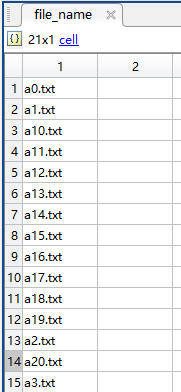
\includegraphics[height=6cm]{disordered_file_name}
        \caption{乱序的文件名}
    \end{minipage}
    \begin{minipage}{0.45\textwidth}
        \centering
        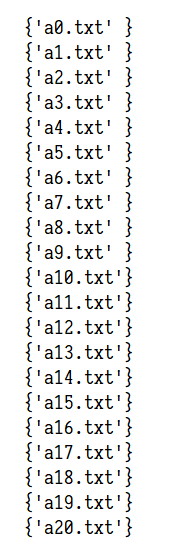
\includegraphics[height=6cm]{ordered_file_name}
        \caption{排序后自然顺序的文件名}
    \end{minipage}
\end{figure}

\section{如何隔行取数据?}

闭上眼睛,想象现在有这样一个数组\mintinline{Matlab}{[1, 2, 3, 4, 5, 6, 7, 8, 9, 10]},我们要隔一列取一个数据,或者隔两列取一个数据。得益于MATLAB的向量化编程,我们可以很方便的做到,

\begin{minted}{Matlab}
mat_a = [1, 2, 3, 4, 5, 6, 7, 8, 9, 10];
mat_b = mat_a(:, 1:2:length(mat_a));
\end{minted}

如果你用循环,那么你的代码就不优雅,另,向量化操作比循环快,大型数组优势明显。以上。

\section{如何在遍历数组的同时删除被遍历过的元素?}

闭上眼睛,想象现在有这样一个数组\mintinline{Matlab}{[1, 2, 3, 4, 5, 6, 7, 8, 9, 10]},我们需要边遍历元素边删除元素。实现方法和Python章节方法一致。

\begin{minted}{Matlab}
mat_a = [1, 2, 3, 4, 5, 6, 7, 8, 9, 10];

while ~isempty(mat_a)
    fprintf("The element being traversed is %d\n", mat_a(1));
    mat_a(1) = [];
    disp(mat_a);
end
\end{minted}




    \chapter{Python}

\section{如何展开一个嵌套的序列?}

我们现在有这样一个序列\mintinline{python}{items = [1, 2, [3, 4, [5, 6, [9, 8], 7], 8]]},我们想逐级展开这个序列,然后将所有元素装入一个序列。

如果这个序列层级较少,我们可以用多层\mintinline{python}{for}循环来遍历这个序列。一旦这个序列超过3层,过多的循环会让你很头疼。同样,这种多层级的问题我们可以用\textbf{递归}来解决。构建一个函数,这个函数能处理第一层的元素,由于第二层是\mintinline{python}{list},它是一个可迭代对象,我们只需要判断第二层是不是可迭代对象,同时忽略\mintinline{python}{str, bytes}对象\footnote{\mintinline{python}{str, bytes}也是可迭代对象,我们要避免其展开成单个字符。}。只要内层是可迭代的,我们就开始递归,对其应用该函数。

\inputminted{python}{code/python/unfold.py}

由于存在递归,所以函数会被调用很多次,每次调用所得的数据都需要保留,如何在多次的调用之间共享保留数据呢?我采用一个默认参数来实现\footnote{前几天没有回想起list有个extend方法,显然用extend方法来实现更加优雅},首次调用时不给默认参数新值,这会产生一个空的\mintinline{python}{list},当对内层对象调用时,将上一次产生的数据赋值给这个参数。输出结果:

\begin{minted}{python}
>>> items1 = ['Paula', ['Thomas', 'Lewis', ['siyu', 'ziyan', ['jianyuan']]]]
>>> items2 = [1, 2, [3, 4, [5, 6, [9, 8], 7], 8]]
>>> items3 = [[1, 2], 3, (4, [5, 6])]
>>> print(unfold(items1))
>>> print(unfold(items2))
>>> print(unfold(items3))
['Paula', 'Thomas', 'Lewis', 'siyu', 'ziyan', 'jianyuan']
[1, 2, 3, 4, 5, 6, 9, 8, 7, 8]
[1, 2, 3, 4, 5, 6]
\end{minted}

但这样做有两个显而易见的坏处,一是当我们的嵌套序列有无限多层,递归会栈溢出;二是序列整个被读取到内存中了,当序列元素非常多,比如1亿,内存会被撑死。坏处一我们不去管他,大多数情况下是适用的,坏处二可以很容易的利用generator来解决\footnote{思路来源~\url{http://python3-cookbook.readthedocs.io/zh_CN/latest/c04/p14_flattening_nested_sequence.html}}。

\inputminted{python}{code/python/unfold_generator.py}

使用generator一来能防止内存爆炸,二来不需要在函数的多次调用见传递数据,代码更清晰明朗。需要注意,generator是惰性序列,边调用边计算,我们需要使用\mintinline{python}{for}迭代出每一个元素或者直接用\mintinline{python}{list()}获取全部元素。

\begin{minted}{python}
items1 = ['Paula', ['Thomas', 'Lewis', ['siyu', 'ziyan', ['jianyuan']]]]
items2 = [1, 2, [3, 4, [5, 6, [9, 8], 7], 8]]
items3 = [[1, 2], 3, (4, [5, 6])]
print(list(unfold(items1)))
print(list(unfold(items2)))
print(list(unfold(items3)))
\end{minted}

\section{如何遍历当前文件夹及其子文件夹中的全部文件?}

前面用MATLAB实现了一个,现在用Python来实现。第一种方法是利用递归来实现,思路同样是先找文件,然后找子文件夹,最后对子文件夹递归;第二种方法是利用os.walk模块,并将其做成generator,这样在应对大量的文件时会有优势。推荐第二种方法,一来os模块考虑了很多我们忽略了的细节\footnote{比如,如果递归版本的函数遍历的根目录是一个磁盘,这个磁盘上的特殊的文件夹“System Volume Information”又是禁止被访问的,这时就会抛出一个PermissionError。笨一点的解决办法是从子目录的list中删除这个目录,好一点的办法就是用os模块了。},二来generator是一个优雅的设计,用Python就应该好好学用generator。

\inputminted{python}{code/python/get_all_file_name.py}

\section{如何在遍历list时删除元素?}

存在一个list\_a = [1, 2, 3, 4, 5, 6, 7, 8, 9],现在需要逐一操作内部元素,并在操作结束之后删除它。使用\mintinline{python}{while}判断\mintinline{python}{list}是否为空,不为空则\mintinline{python}{pop}第一个元素,在循环下依次操作每一个元素。

\begin{minted}{python}
list_a = [1, 2, 3, 4, 5, 6, 7, 8, 9]

while list_a:
    temp = list_a.pop(0)
    print(temp)
\end{minted}

    \chapter{C和C++}

\section{C语言的动态数组}

大多数时候为了方便(其实是我菜),会使用库较多(方便)的C++,但是C语言在实际生产中使用率仍然很高,比如长期使用的ANSYS Fluent的UDF就不得不用C语言。下面是一个简易的动态数组的实现,来源\footnote{\url{https://stackoverflow.com/questions/3536153/c-dynamically-growing-array}}。

\begin{minted}{c}
#include <iostream>

typedef struct
{
    int *array;
    size_t used;
    size_t size;
} Array;

void initArray(Array *a, size_t initialSize)
{
    a->array = (int *)malloc(initialSize * sizeof(int));
    a->used = 0;
    a->size = initialSize;
}

void insertArray(Array *a, int element)
{
    // a->used is the number of used entries, because a->array[a->used++] updates a->used only *after* the array has been accessed.
    // Therefore a->used can go up to a->size
    if (a->used == a->size)
    {
        a->size *= 2;
        a->array = (int *)realloc(a->array, a->size * sizeof(int));
    }
    a->array[a->used++] = element;
}

void freeArray(Array *a)
{
    free(a->array);
    a->array = NULL;
    a->used = a->size = 0;
}

int main()
{
    Array a;
    int i;

    initArray(&a, 5); // initially 5 elements
    for (i = 0; i < 100; i++)
        insertArray(&a, i);     // automatically resizes as necessary
    printf("%d\n", a.array[9]); // print 10th element
    printf("%d\n", a.used);     // print number of elements
    freeArray(&a);
    return 0;
}

\end{minted}
    \chapter{算法}

算法可视化的网站,\url{https://www.cs.usfca.edu/\%7Egalles/visualization/Algorithms.html},晕乎乎的时候看几遍动画就明白了。

\section{排序}

先来了解几个基本概念:

排序:将一组“无序”的记录序列调整为“有序”的记录序列。

稳定性:假定在待排序的记录序列中,存在多个具有相同的关键字的记录,若经过排序,这些记录的相对次序保持不变,则称这种排序算法是稳定的,否则称为不稳定的。

排序算法的分类:插入类、交换类、选择类、归并类和基数类。

基于⽐较的排序算法的最佳性能为$ O(n\log n) $。

\subsection{冒泡排序}

复杂度:$ O(n^2) $

1、对数组array[n]进行从0~n-1项的扫描,每碰到相邻两项数值大的在前小的在后时,对二者进行交换。当扫描进行完成后,0~n-1中最大的元素必然已经在array[n-1]就位,而所有数值较小,序号却靠后的元素,序号也减小了1。

2、既然最大的元素已在array[n-1]的位置就位,接下来的扫描只需从0~n-2。具体过程同1。同样的,扫描结束后0~n-2中最大的元素(全数组第二大的元素)必然已经在array[n-2]就位,而所有数值较小,序号却靠后的元素,序号也减小了1。

3、如此不断重复,直到最小的元素在array[0]的位置就位。

从上述描述中我们可以看到“冒泡排序”这个名字的由来:每一次扫描,都可以使得数值较小,序号却靠后的元素的序号减少1,宏观来看这些元素就像是从数组底部向上慢慢上浮的泡泡。

\inputminted{c++}{code/algorithm/bubble_sort.cpp}

\subsection{插入排序}

复杂度:$ O(n^2) $,具体算法描述如下:

1.从第一个元素开始,该元素可以认为已经被排序

2.取出下一个元素,在已经排序的元素序列中\textit{从后向前扫描}

3.如果该元素(已排序)大于新元素,将该元素移到下一位置

4.重复步骤3,直到找到已排序的元素小于或者等于新元素的位置

5.将新元素插入到该位置后

6.重复步骤2~5

插入排序和人们打牌时所用的排序方式类似:抽第一张牌,此时手上的牌只有一张,所以是有序的。再抽一张牌,和手上的那张牌的大小进行比较,比它大就放在后面,否则放在前面。再抽一张牌,和手上的牌进行比较,插入在合适的位置,保持手上的牌有序。不断重复,直到牌抽完。从宏观来看,插入排序把数组分割成两部分,\textit{前段有序后段无序},随着插入排序的进行,后段无序的牌也越来越少,直到后段全部融入前段,排序也就结束了。

\inputminted{c++}{code/algorithm/insert_sort.cpp}

\subsection{归并排序}

复杂度:$ O(n\log n) $

归并排序的操作有两步,分割和归并

1、分割:将数组二等分,并将得到的子数组继续二等分,直到每个子数组只剩下一个元素为止。

2、归并:不断将原本属于同一个数组的两个子数组归并成一个有序的数组,方法为不断比较子数组的首元素,并弹出较小的放入合并后组成的数组中。直到所有子数组合并为一个数组。

\subsection{选择排序}

复杂度:$ O(n^2) $

在未排序序列中找到最小(大)元素,存放到排序序列的起始位置,然后,再从剩余未排序元素中继续寻找最小(大)元素,然后放到已排序序列的末尾。以此类推,直到所有元素均排序完毕。

\inputminted{cpp}{code/algorithm/select_sort.cpp}

\subsection{快速排序}

复杂度:$ O(n^2) $(最坏情况);$ O(n\log n) $(平均情况)

1、从数组中随机选出一个元素,和数组首元素互换位置,并记下其大小。

2、使用两个指针,指针a指向数组头,指针b指向数组尾。

3、指针b从后向前扫描,找到一个数比选出元素小时,暂停,将其值保存在指针a所指的位置中。

4、指针a从前往后扫描,找到一个数比选出元素大时,暂停,将其值保存在指针b所指的位置中。

5、循环重复3、4,直到a<b不再成立。

6、将选出元素放在指针a、b同时指向的位置,并用此位置将数组分割成前后不包含选出元素的两个子数组,对子数组进行步骤1~6。
    \chapter{Git}

\section{如何给Git仓库添加一个空文件夹?}
默认情况下,空文件夹不被记录,也不能被推送。特殊需求参见\href{https://stackoverflow.com/questions/115983/how-can-i-add-an-empty-directory-to-a-git-repository}{How can I add an empty directory to a Git repository? - Stack Overflow}


    \backmatter
\end{document}